\subsection{Nabolister}
En måde at repræsentere en graf på er ved at lave en \emph{naboliste}. Nabolister er tabeller, der giver en oversigt over hvilke knuder, der er naboer. Dog vil man ikke kunne se, hvis der er parallelle kanter. En naboliste er bygget op således, at knuden, man vil beskrive, er i venstre side af tabellen, og naboknuderne er skrevet i højre side. \\

\begin{figure}[h]
  \centering
  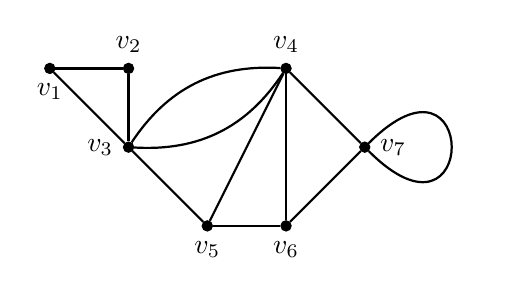
\begin{tikzpicture}
\tikzset{enclosed/.style={draw, circle, inner sep=0pt, minimum size=.13cm, fill=black}}
    \node[enclosed] at (1,2) (v2) [label=above:\(v_2\)] {};
    \node[enclosed] at (3,2) (v4) [label=above:\(v_4\)] {};
    \node[enclosed] at (4,1) (v7) [label=right:\(v_7\)] {};
    \node[enclosed] at (2,0) (v5) [label=below:\(v_5\)] {};
    \node[enclosed] at (3,0) (v6) [label=below:\(v_6\)] {};
    \node[enclosed] at (1,1) (v3) [label=left:\(v_3\)] {};
    \node[enclosed] at (0,2) (v1) [label=below:\(v_1\)] {};
    
    \path[thick] (v1) edge node[midway, above] {} (v2);
    \path[thick] (v4) edge[bend right] node[midway, above] {} (v3);
    \path[thick] (v3) edge node[midway, above] {} (v2);
    \path[thick] (v3) edge[bend right] node[midway, above] {} (v4);
    \path[thick] (v4) edge node {} (v5);
    \path[thick] (v4) edge node {} (v6);
    \path[thick] (v4) edge node {} (v7);
    \path[thick] (v7) edge node {} (v6);
    \path[thick] (v6) edge node {} (v5);
    \path[thick] (v5) edge node {} (v3);
    \path[thick] (v1) edge node {} (v3);
    \path[thick] (v7) edge [out=315,in=45,looseness=50] node[right] {} (v7);


  \end{tikzpicture}
  \caption{Ikke-orienteret pseudograf.}
  \label{fig:ikke-orienteret-pseudo}
\end{figure}


\begin{table}[h]
	\centering
	\begin{tabular}{ |p{3cm}|p{3cm}|}
 		\hline
 		Knuder & Naboknuder\\
 		\hline
 		$v_1$ & $v_2$, $v_3$\\
		$v_2$ & $v_1$, $v_3$ \\
		$v_3$ & $v_1$, $v_2$, $v_4$, $v_5$ \\
		$v_4$ & $v_1$, $v_3$, $v_5$, $v_7$ \\
		$v_5$ & $v_3$, $v_4$, $v_6$ \\
		$v_6$ & $v_4$, $v_5$, $v_7$ \\
		$v_7$ & $v_4$, $v_6$, $v_7$ \\
 		\hline 
	\end{tabular}
	\caption{Naboliste til figur \ref{fig:ikke-orienteret-pseudo}.}
	\label{tab:naboliste-ikke-orienteret}
\end{table}



Ud fra \autoref{tab:naboliste-ikke-orienteret} ses, at knuden $v_4$ har naboknuderne $v_3$,$v_5$,$v_1$ og $v_7$ men man kan ikke se, at der er en ekstra kant mellem $v_4$ og $v_3$. Man kan dog se, at $v_7$ har en løkke, da den er nabo til sig selv.

\begin{figure}[H]
  \centering
  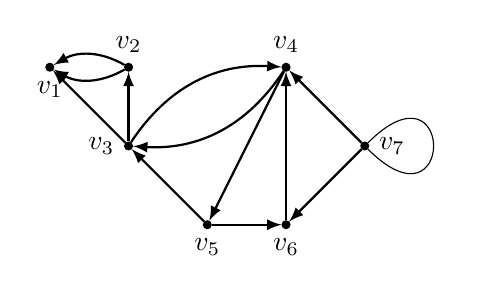
\begin{tikzpicture}[every loop/.style={}]
      \tikzset{enclosed/.style={draw, circle, inner sep=0pt, minimum size=.10cm, fill=black}}
    \node[enclosed] at (1,2) (v_2) [label=above:\(v_2\)] {};
    \node[enclosed] at (3,2) (v_4) [label=above:\(v_4\)] {};
    \node[enclosed] at (4,1) (v_7) [label=right:\(v_7\)] {};
    \node[enclosed] at (2,0) (v_5) [label=below:\(v_5\)] {};
    \node[enclosed] at (3,0) (v_6) [label=below:\(v_6\)] {};
    \node[enclosed] at (1,1) (v_3) [label=left:\(v_3\)] {};
    \node[enclosed] at (0,2) (v_1) [label=below:\(v_1\)] {};

    \footnotesize
    	\path[->, > = latex, thick] (v_2) edge[bend right] node {} (v_1);
    	\path[->, > = latex, thick] (v_2) edge[bend left] node {} (v_1);
    	\path[->, > = latex, thick] (v_3) edge[bend left] node {} (v_4);
    	\path[->, > = latex, thick] (v_3) edge node {} (v_2);
    	\path[->, > = latex, thick] (v_4) edge[bend left] node {} (v_3);
    	\path[->, > = latex, thick] (v_4) edge node {} (v_5);
   		\path[->, > = latex, thick] (v_6) edge node {} (v_4);
		\path[->, > = latex, thick] (v_7) edge node {} (v_4);
		\path[->, > = latex, thick] (v_7) edge node {} (v_6);
		\path[->, > = latex, thick] (v_5) edge node {} (v_6);
		\path[->, > = latex, thick] (v_5) edge node {} (v_3);
		\path[->, > = latex, thick] (v_3) edge node {} (v_1);
		\path (v_7) edge [out=315,in=45,looseness=50] node {} (v_7);




  \end{tikzpicture}
  \caption{Orienteret multigraf.}
  \label{fig:orienteretmulti}
\end{figure}

\begin{table} [H]

	\centering
	\begin{tabular}{ |p{3cm}|p{3cm}|}
 		\hline
 		Knuder & Naboknuder\\
 		\hline
 		$v_1$ & \\
		$v_2$ & $v_1$ \\
		$v_3$ & $v_1$, $v_2$, $v_4$ \\
		$v_4$ & $v_3$, $v_5$, \\
		$v_5$ & $v_3$, $v_6$ \\
		$v_6$ & $v_4$ \\
		$v_7$ & $v_4$, $v_6$, $v_7$ \\
 		\hline
	\end{tabular}
\caption{Naboliste til figur \ref{fig:orienteretmulti}.}
\label{tab:nabolisteorienteret}
\end{table}
Tabel \ref{tab:nabolisteorienteret} viser en oversigt over den orienterede grafs (Figur \ref{fig:orienteretmulti}) naboknuder. Kigger man på $v_3$ og $v_4$ i tabellen, kan man se, at der er parallelle kanter, da kanterne er orienteret i hver deres retning. Kigger man på $v_1$ og $v_2$, kan man ikke se, at der er parallelle kanter mellem $v_1$ og $v_2$, da begge kanter er orienteret fra $v_2$ til $v_1$. Naboknuderne går også under fællesbetegnelsen nabolag. Et nabolag er defineret ved:

\begin{defn}[Nabolag] \label{defn:nabolag}
Knuden $v$'s \emph{nabolag}, $N(v)$, er en betegnelse for alle naboer til knuden, $v$, i grafen, $G=(V,E)$. Når $A \subseteq V$, er $N(A)$ betegnelsen for alle naboer til mindst én knude i $A$.
\end{defn}

Antallet af knuder i et nabolag, er også knudens grad, medmindre der er tale om en knude med en løkke, se \autoref{sec:grader}. 
På samme måde som i nabolister, kan nabolag også ses i nabomatricer.